\documentclass[11pt,a4paper]{article}
\usepackage[T1]{fontenc}
\usepackage{lmodern}
\usepackage[margin=26mm]{geometry}
\usepackage{amsmath,amssymb,amsthm,mathtools}
\usepackage{microtype,booktabs,longtable,array,graphicx}
\usepackage{enumitem,fancyhdr}
\usepackage{xurl}
\usepackage[hidelinks]{hyperref}
\usepackage[nameinlink,noabbrev]{cleveref}
\hypersetup{pdftitle={Spectral Collisions and Boundary Asymptotics for Zig-zag Eulerian Numbers},
 pdfauthor={Research report prepared for Vladimir Reshetnikov},
 pdfsubject={OEIS A205497; exact minimal recurrences; uniform asymptotics; log-concavity}}
\pagestyle{fancy}
\fancyhf{}
\fancyhead[L]{\small Zig-zag Eulerian numbers}
\fancyhead[R]{\small Research report \textbar\ 1 October 2026}
\fancyfoot[C]{\thepage}
\setlength{\headheight}{14pt}
\setlength{\parskip}{4pt}
\setlength{\parindent}{1.2em}
\setlist{itemsep=3pt,topsep=5pt}
\emergencystretch=2em
\allowdisplaybreaks[1]
\newtheorem{theorem}{Theorem}[section]
\newtheorem{proposition}[theorem]{Proposition}
\newtheorem{lemma}[theorem]{Lemma}
\newtheorem{corollary}[theorem]{Corollary}
\theoremstyle{definition}
\newtheorem{definition}[theorem]{Definition}
\newtheorem{remark}[theorem]{Remark}
\newcommand{\Om}{\Omega}
\newcommand{\one}{\mathbf{1}}
\newcommand{\N}{\mathbb{N}}
\newcommand{\Z}{\mathbb{Z}}
\newcommand{\Q}{\mathbb{Q}}
\newcommand{\R}{\mathbb{R}}
\newcommand{\C}{\mathbb{C}}
\DeclareMathOperator{\lcm}{lcm}
\DeclareMathOperator{\des}{des}
\DeclareMathOperator{\ord}{ord}
\DeclareMathOperator{\spec}{spec}
\newcommand{\eps}{\varepsilon}
\newcommand{\abs}[1]{\left|#1\right|}
\title{\vspace{-1.2cm}\textbf{Spectral Collisions and Boundary Asymptotics\\for Zig-zag Eulerian Numbers}\\[0.5em]
\large Exact minimal recurrences, a crossover law, and growing-edge log-concavity\\for OEIS A205497}
\author{Research report prepared for Vladimir Reshetnikov}
\date{1 October 2026}
\begin{document}
\maketitle
\thispagestyle{empty}
\begin{abstract}
Let $z(n,k)$ count linear extensions with $k$ descents of a naturally labeled
$n$-element fence poset.  We study the fixed-column sequences
$M_{i,k}=z(i+k+2,k)$ and the regime in which $k$ increases with $n$.
Starting from established order-polynomial and unit-primitive-matrix formulas,
we determine the \emph{exact reduced denominator} of every column generating
function.  A complete classification of shared eigenvalues gives its degree
$r_k$ by a totient sum and yields
\[
 r_k=\frac{40}{27\pi^2}(k+1)^3+O(k^2\log(k+2)).
\]
Thus the minimal recurrence has asymptotically $80/(9\pi^2)$ of the order of
the familiar unreduced recurrence.
We next obtain an explicit uniform relative-error bound for the leading
spectral approximation.  At the transition
$n/(k+3/2)-\log n\to s$, its relative correction tends to
$\exp(-e^{-s})$.  Finally, for every fixed $0<c<1/2$, all sufficiently large
rows are strictly log-concave at every index
$1\le k\le c n/\log n-2$, and at the reflected right-edge indices.
These are not proofs of full-row log-concavity or real-rootedness.
The report separates prior results from the additional theorems, records two
OEIS presentation corrections, and supplies exact rational certificates,
independent finite enumeration checks, and a further research program.
\end{abstract}
\vfill
\noindent\textbf{Status.} This is an unrefereed mathematical research manuscript with
ordinary proofs and reproducible calculations.  It is not a Lean formalization.
The repository and OEIS entries were not modified.  A targeted literature
search is not an exhaustive priority certification.
\newpage
\begingroup
\small
\setlength{\parskip}{0pt}
\tableofcontents
\endgroup
\newpage

\section{The problem and the contribution}
\label{zz:sec:intro}
The zig-zag Eulerian triangle is a particularly suitable OEIS research target:
it combines a concrete permutation statistic, rational generating functions,
explicit matrix spectra, and a genuine outstanding shape conjecture.
Throughout this report, $\log$ is the natural logarithm, and all asymptotic
statements concern positive integers tending to infinity unless otherwise stated.

\subsection{What was already known}
OEIS A205497 records the triangle $z(n,k)$, its older rectangular arrangement
$M_{i,k}$, and several statements still labeled conjectures \cite{oeis205497}.
Those labels must not be read as evidence that all those statements remain
unproved.  Xin and Zhong's paper \cite{xz}, especially Section~5, already
establishes the fixed-column rational formulas and their Perron growth rates.
Their Remark~5.7 explicitly observes cancellation in a displayed denominator.
Petersen and Zhuang \cite{pz} develop the descent interpretation, order
polynomials, gamma-nonnegativity, and a refined theory.  Their
Conjecture~6.1 includes full-row log-concavity and real-rootedness.

The results attributed to these papers are the starting point, not claims of
new discovery.  In particular, finding a proof of an old OEIS formula would
not, by itself, constitute a new theorem here.

\subsection{The additional questions answered here}
The main algebraic question is sharper than rationality:
\begin{quote}
Which factors and multiplicities actually survive after every cancellation,
and what is the \emph{smallest} constant-coefficient recurrence for a column?
\end{quote}
The main analytic question is sharper than fixed-$k$ asymptotics:
\begin{quote}
How far toward the interior may $k$ grow while spectral asymptotics remain
uniform, and can those estimates establish a growing part of the
log-concavity conjecture?
\end{quote}
The answers are summarized below.  Here
\[
 H_m=(\mathbf{1}_{\{i+j\ge m+1\}})_{1\le i,j\le m},\qquad
 D_m(x)=\det(I-xH_m),\qquad D_0=1.
\]
All polynomial greatest common divisors and least common multiples are
normalized to have constant coefficient~$1$.

\begin{theorem}[Main algebraic result]
\label{zz:thm:main-alg}
For every $k\ge0$, the reduced denominator of
$C_k(x)=\sum_{i\ge0}M_{i,k}x^i$ is exactly
\begin{equation}\label{zz:eq:main-lcm}
 R_k(x)=\lcm_{1\le m\le k+1}D_m(x)^{k+2-m}.
\end{equation}
Its degree $r_k$ is the minimum possible order of a homogeneous
constant-coefficient recurrence, even when the recurrence is required only
eventually.  An explicit totient formula is given in
\cref{zz:thm:degree}; in particular,
\begin{equation}\label{zz:eq:main-order}
 r_k=\frac{40}{27\pi^2}(k+1)^3+O\bigl((k+1)^2\log(k+2)\bigr).
\end{equation}
For $k\ge1$, the reduced numerator has degree $r_k-k-3$.
\end{theorem}

\begin{theorem}[Main analytic results]
\label{zz:thm:main-analysis}
Put
\begin{equation}\label{zz:eq:rho-alpha-intro}
 t_m=\frac{\pi}{4m+2},\qquad
 \rho_m=\frac{1}{2\sin t_m},\qquad
 \alpha_m=\frac{4\rho_m\cos^2t_m}{2m+1}.
\end{equation}
Then:
\begin{enumerate}[label=(\roman*)]
\item For every fixed $0<c<1$,
$z(n,k)\sim\alpha_{k+1}\rho_{k+1}^{\,n}$ uniformly over
$0\le k$ with $k+1\le c n/\log n$.
\item If $n/(k+3/2)-\log n\to s\in\R$, then
\begin{equation}\label{zz:eq:main-crossover}
 \frac{z(n,k)}{\alpha_{k+1}\rho_{k+1}^{\,n}}
 \longrightarrow \exp(-e^{-s}).
\end{equation}
\item For every fixed $0<c<1/2$, all sufficiently large $n$ satisfy
\begin{equation}\label{zz:eq:main-lc}
 z(n,k)^2>z(n,k-1)z(n,k+1)
 \quad\text{whenever}\quad 1\le k,\quad k+2\le\frac{cn}{\log n}.
\end{equation}
The same holds at the reflected indices $n-2-k$.
\end{enumerate}
\end{theorem}

The claims presented as additional contributions are the exact minimality and
collision classification, the resulting recurrence-order asymptotic, and the
uniform, crossover, and growing-edge theorems.  The proofs below establish
these statements within this manuscript.  Their global bibliographic novelty
has not been independently certified.

\subsection{Relation to ProveIt}
The requested repository is a natural destination for a proof-and-certificate
package of this kind.  Its README distinguishes exploratory computations from
formal theorem boundaries \cite{proveit}.  We follow that distinction: the
proofs below do not assume any unverified research claim from the repository,
and the Python certificates do not masquerade as kernel-checked proofs.
The contribution is standalone and ready for review or later formalization,
not a claim that the repository already contains these results.

\emph{[Write note, batch 73O2, 1 October 2026.]} This manuscript is
placed in ProveIt as the report \texttt{a205497-zigzag-eulerian-spectra}
(Section~\ref{zz:sec:provenance}). The repository contains no other work on
A205497 or on fence linear extensions. Its volume \emph{Combinatorial
Transseries and Their Inverses} \cite{cti} treats two related but different
objects: the Euler zigzag numbers A000111 (its chapter \texttt{ct:ch:zigzag} on
alternating permutations), which are the row sums $\sum_kz(n,k)$ of A205497, and the
columns of the classical Eulerian triangle A008292 (its proposition
\texttt{t1:prop:eulerian}). A205497 is the descent refinement of the linear
extensions of the fence, not either of those; nothing here depends on, or
is implied by, that volume.

\section{Definitions and the order-polynomial bridge}
\label{zz:sec:definitions}
Let $P_n$ be the fence poset with underlying vertices
$v_1,\ldots,v_n$ and relations
\[
 v_1<v_2>v_3<v_4>\cdots.
\]
Choose any natural labeling: a bijection to $[n]$ that respects every poset
comparison.  For a linear extension, written as a permutation of its labels,
let $\des$ be its number of adjacent descents.  Define
\[
 A_n(t)=\sum_k z(n,k)t^k.
\]
For $n=0$ set $A_0(t)=1$.  This convention also gives
$A_1(t)=A_2(t)=1$.  For $n\ge2$, the degree is $n-2$, and the established
symmetry is
\begin{equation}\label{zz:eq:symmetry}
 z(n,k)=z(n,n-2-k).
\end{equation}
We use this known symmetry only to transfer left-edge statements to the
right edge.  All left-edge analysis is independent of it.

\begin{definition}
For $m\ge1$, let $\Om_n(m)$ count words $a_1\cdots a_n$ over $[m]$ with
\[
 a_1\le a_2\ge a_3\le a_4\ge\cdots.
\]
Set $\Om_0(m)=1$.  These are precisely the order-preserving maps
$P_n\to[m]$.  (The array of these counts is OEIS A050446 \cite{oeis50446},
up to the indexing conventions reconciled in \cite{pz,xz}.)
\end{definition}

\begin{proposition}[Order-polynomial identity]
\label{zz:prop:p-partitions}
For every $n\ge0$,
\begin{equation}\label{zz:eq:p-partition}
 \frac{tA_n(t)}{(1-t)^{n+1}}=\sum_{m\ge1}\Om_n(m)t^m.
\end{equation}
Consequently, for every $k\ge0$,
\begin{equation}\label{zz:eq:extraction}
 z(n,k)=\sum_{j=0}^{k}(-1)^j\binom{n+1}{j}\Om_n(k+1-j),
\end{equation}
where $\binom{n+1}{j}=0$ for $j>n+1$.
\end{proposition}
\begin{proof}
Sort the vertices by the value of an order-preserving map, breaking equalities
by increasing natural label.  The result is a unique linear extension.
Along a fixed extension with $d$ descents, the values form a weakly increasing
sequence in $[m]$, with a compulsory strict increase at each descent.
Subtracting the number of preceding compulsory increases gives
$\binom{m+n-1-d}{n}$ possibilities, interpreted as zero when $m\le d$.
The generating function of these numbers over $m\ge1$ is
$t^{d+1}/(1-t)^{n+1}$.  Summing over extensions proves
\eqref{zz:eq:p-partition}.  The case $n=0$ follows from the geometric series.
Multiplication by $(1-t)^{n+1}$ and coefficient extraction prove
\eqref{zz:eq:extraction}.
\end{proof}

This is the standard $P$-partition mechanism; its use for this triangle and
the equivalent interpretation by big returns of alternating permutations are
established in \cite{pz}.  A big return is a pair of consecutive values
$i,i+1$ for which the position of $i$ exceeds that of $i+1$ by more than~$1$.
That interpretation will supply an independent finite check.

\begin{center}
\begin{tabular}{cl}
\toprule
$n$ & $(z(n,0),z(n,1),\ldots)$\\
\midrule
2 & $1$\\
3 & $1,1$\\
4 & $1,3,1$\\
5 & $1,7,7,1$\\
6 & $1,14,31,14,1$\\
7 & $1,26,109,109,26,1$\\
8 & $1,46,334,623,334,46,1$\\
\bottomrule
\end{tabular}
\end{center}
The indexing distinction is essential:
\begin{equation}\label{zz:eq:indexing}
 M_{i,k}=z(i+k+2,k),\qquad
 C_k(x)=\sum_{i\ge0}z(i+k+2,k)x^i.
\end{equation}
If $B_k(x)=\sum_{n\ge0}z(n,k)x^n$, then
\begin{equation}\label{zz:eq:shift}
 C_k(x)=x^{-k-2}B_k(x)\quad(k\ge1),\qquad
 C_0(x)=B_0(x)=\frac1{1-x}.
\end{equation}
For $k\ge1$, all the apparently negative powers in the first expression
vanish.  The separate $k=0$ formula prevents a spurious boundary error.

\section{A complete spectral expansion}
\label{zz:sec:spectrum}
The spectrum of the unit-primitive matrix is known; see \cite{xz}.
We give a proof including the endpoint weights needed for uniform estimates
and for excluding pole cancellation.

\begin{lemma}[The walk model]
\label{zz:lem:walk}
For $n\ge1$,
\begin{equation}\label{zz:eq:walk}
 \Om_n(m)=\one^T H_m^{n-1}\one.
\end{equation}
Moreover, $H_m$ is invertible,
$H_m^{-1}\one=e_m$, and $(H_m^2)_{ij}=\min(i,j)$.
\end{lemma}
\begin{proof}
Reflect each odd-position letter of a weak alternating word:
$b_i=m+1-a_i$ for odd $i$, and $b_i=a_i$ for even $i$.
Every adjacent inequality becomes $b_i+b_{i+1}\ge m+1$.
Thus the transformed word is a walk counted by \eqref{zz:eq:walk}.
Let $L$ be the lower-triangular all-ones matrix and $J$ the reversal matrix.
Then $H_m=LJ$, so $\det H_m=\det J=\pm1$.
The last column of $H_m$ is $\one$, giving $H_m^{-1}\one=e_m$.
Finally, the $(i,j)$ entry of $H_m^2$ counts the indices
$r\ge\max(m+1-i,m+1-j)$, of which there are $\min(i,j)$.
\end{proof}

\begin{theorem}[Spectrum with nonzero weights]
\label{zz:thm:spectral}
For $1\le r\le m$, put
\[
 \theta_{m,r}=\frac{(2r-1)\pi}{2m+1},\qquad
 \lambda_{m,r}=\frac{(-1)^{r+1}}{2\sin(\theta_{m,r}/2)},\qquad
 c_{m,r}=\frac{4\lambda_{m,r}\cos^2(\theta_{m,r}/2)}{2m+1}.
\]
The $\lambda_{m,r}$ are the distinct eigenvalues of $H_m$ and are arranged in
strictly decreasing absolute value.  Every $c_{m,r}$ is nonzero, and
\begin{equation}\label{zz:eq:full-spectrum}
 \Om_n(m)=\sum_{r=1}^m c_{m,r}\lambda_{m,r}^{\,n}
 \quad(n\ge0).
\end{equation}
Furthermore,
\begin{equation}\label{zz:eq:weight-sums}
 \sum_r c_{m,r}=1,\qquad \sum_r\frac{c_{m,r}}{\lambda_{m,r}}=1.
\end{equation}
\end{theorem}
\begin{proof}
The inverse of $(\min(i,j))_{i,j=1}^m$ is the tridiagonal matrix with
$-1$ on the neighboring off-diagonals, diagonal entries $2$ except for the
last entry~$1$.  The vectors
\[
 v_r(i)=\sin(i\theta_{m,r})
\]
are its eigenvectors: the usual second-difference identity applies with
boundary conditions $v_r(0)=0$ and $v_r(m+1)=v_r(m)$.
Its eigenvalues are $4\sin^2(\theta_{m,r}/2)$ and are distinct.
Since $H_m$ commutes with its inverse square, it preserves each of these
one-dimensional eigenspaces.  To determine the sign of its eigenvalue, use
\[
 \sum_{i=1}^m\sin(i\theta_{m,r})
 =\frac12\cot(\theta_{m,r}/2),\qquad
 v_r(m)=(-1)^{r-1}\cos(\theta_{m,r}/2).
\]
The quotient is exactly $\lambda_{m,r}$.
Also,
\[
 \|v_r\|^2=\sum_{i=1}^m\sin^2(i\theta_{m,r})=\frac{2m+1}{4}.
\]
For example, the last identity follows by summing the nontrivial
$(2m+1)$st roots of unity in symmetric pairs.
Orthogonal spectral decomposition of \eqref{zz:eq:walk} now gives
\[
 \one^TH_m^{n-1}\one
 =\sum_r\frac{(\one^Tv_r)^2}{\|v_r\|^2}\lambda_{m,r}^{n-1},
\]
whose coefficient after extracting $\lambda_{m,r}^n$ is $c_{m,r}$.
Invertibility permits the same expression at $n=0$, because
$\one^TH_m^{-1}\one=\one^Te_m=1$.
Likewise,
$\one^TH_m^{-2}\one=\|H_m^{-1}\one\|^2=1$, proving the second
identity in \eqref{zz:eq:weight-sums}.  Nonvanishing and the ordering of absolute
values follow directly from the trigonometric expressions.
\end{proof}

The Perron eigenvalue and its coefficient are
$\lambda_{m,1}=\rho_m$ and $c_{m,1}=\alpha_m$ as in
\eqref{zz:eq:rho-alpha-intro}.
For $F_m(x)=\sum_{n\ge0}\Om_n(m)x^n$, the theorem gives
\begin{equation}\label{zz:eq:F-spectrum}
 F_m(x)=\sum_{r=1}^m\frac{c_{m,r}}{1-\lambda_{m,r}x}.
\end{equation}
Every pole is present, so its reduced denominator is $D_m$.
The numerator has degree $m-1$, and \eqref{zz:eq:weight-sums} gives
\begin{equation}\label{zz:eq:F-infinity}
 F_m(x)=-x^{-1}+O(x^{-2})\qquad(x\to\infty).
\end{equation}

For efficient exact computation we also use the established identity
$F_m(x)=1/(F_{m-1}(-x)-x)$, $m\ge2$ \cite[Theorem~3.15]{pz}.
Combined with the pole count above, induction yields
\begin{equation}\label{zz:eq:D-recurrence}
 D_0=1,\quad D_1=1-x,\quad
 D_m(x)=D_{m-2}(x)-xD_{m-1}(-x),\qquad
 F_m(x)=\frac{D_{m-1}(-x)}{D_m(x)}.
\end{equation}
There can be no canceled factor in this induction, since the reduced
denominator already has degree~$m$.

\section{Exact column formulas and minimality}
\label{zz:sec:minimal}
Combining \eqref{zz:eq:extraction} and \eqref{zz:eq:full-spectrum} gives an exact,
finite expression rather than only an asymptotic expansion.
\begin{proposition}[Exponential-polynomial expression]
\label{zz:prop:exp-poly}
For $n,k\ge0$,
\begin{equation}\label{zz:eq:exp-poly}
 z(n,k)=\sum_{m=1}^{k+1}\sum_{r=1}^m
 (-1)^{k+1-m}c_{m,r}
 \binom{n+1}{k+1-m}\lambda_{m,r}^{\,n}.
\end{equation}
\end{proposition}
This formula is a consequence of the established spectral and extraction
formulas.  Its useful feature for the new minimality question is that a shared
eigenvalue may occur at several sizes, but the polynomial multipliers then
have \emph{different degrees}.

For $j\ge0$ define
\begin{equation}\label{zz:eq:Psi}
 \Psi_0(u)=\frac1{1-u},\qquad
 \Psi_j(u)=\frac{u^{j-1}}{(1-u)^{j+1}}\quad(j\ge1).
\end{equation}
The binomial-series identity
$\sum_{n\ge0}\binom{n+1}{j}u^n=\Psi_j(u)$ gives
\begin{equation}\label{zz:eq:B-explicit}
 B_k(x)=\sum_{m=1}^{k+1}\sum_{r=1}^m
 (-1)^{k+1-m}c_{m,r}\Psi_{k+1-m}(\lambda_{m,r}x).
\end{equation}
Alternatively, setting $\vartheta=x\,d/dx$,
\begin{equation}\label{zz:eq:B-differential}
 B_k(x)=\sum_{j=0}^k(-1)^j\binom{\vartheta+1}{j}F_{k+1-j}(x).
\end{equation}
The operator binomial is a polynomial in $\vartheta$, divided by $j!$.
Both identities hold as formal rational identities.

\begin{proof}[Proof of the exact-denominator assertion in \cref{zz:thm:main-alg}]
Fix an eigenvalue $\lambda$ occurring among sizes $1,\ldots,k+1$.
In \eqref{zz:eq:B-explicit}, its occurrence at size $m$ has a pole of order
$j+1=k+2-m$ at $x=1/\lambda$.
The numerator of $\Psi_j$ is $1$ at that point, and the coefficient $c_{m,r}$
is nonzero.  Within one size, all eigenvalues are distinct.
Among all sizes sharing $\lambda$, the smallest size $m_0$ therefore
contributes a \emph{unique} highest-order pole.  Lower-order terms cannot
cancel it.  Its order is exactly $k+2-m_0$, the maximum of the exponents
assigned to that root by the factors in \eqref{zz:eq:main-lcm}.
This proves the denominator formula for $B_k$.  For $k\ge1$, multiplication
by $x^{-k-2}$ neither removes nor changes any nonzero pole, and the origin is
removable by \eqref{zz:eq:shift}.  The $k=0$ case is direct.
\end{proof}

\begin{lemma}[Denominators and recurrence order]
\label{zz:lem:rec-order}
Let $C(x)=N(x)/R(x)$ with $N,R\in\Q[x]$, $R(0)=1$,
$\gcd(N,R)=1$, and $\deg N<\deg R=r$.
Then the coefficient sequence satisfies a recurrence of order~$r$.
No recurrence of smaller order can hold for all sufficiently large indices,
even with complex coefficients.
\end{lemma}
\begin{proof}
Write $R=1+r_1x+\cdots+r_rx^r$.  Comparing coefficients of $RC=N$ gives
$a_i+r_1a_{i-1}+\cdots+r_ra_{i-r}=0$ for $i\ge r$.
If a polynomial $Q$ encoding an eventual recurrence had smaller degree,
then $QC$ would be a polynomial, since only finitely many recurrence residuals
would be nonzero.  Thus $R$ would divide $Q$ after reduction, a contradiction.
Equivalently, every pole of $C$ and its full multiplicity must be canceled by
$Q$.  This latter argument also covers complex recurrence coefficients.
\end{proof}

\begin{proposition}[Numerator degree]
\label{zz:prop:numdegree}
Let
\[
 \mathcal P_k(x)=\prod_{m=1}^{k+1}D_m(x)^{k+2-m}.
\]
For $k\ge1$, writing $C_k=N_k/R_k=G_k/\mathcal P_k$, one has
\begin{align}
 \deg N_k&=r_k-k-3,\label{zz:eq:reduced-num}\\
 \deg G_k&=\binom{k+3}{3}-k-3
          =\frac{(k-1)(k+3)(k+4)}6.\label{zz:eq:old-num}
\end{align}
Moreover, $C_k(x)=-x^{-k-3}+O(x^{-k-4})$ at infinity.
\end{proposition}
\begin{proof}
In \eqref{zz:eq:B-explicit}, all terms with $j\ge1$ are $O(x^{-2})$ at infinity.
The $j=0$ terms form $F_{k+1}(x)$, which is $-x^{-1}+O(x^{-2})$ by
\eqref{zz:eq:F-infinity}.  Use \eqref{zz:eq:shift}.  The asserted degrees follow
from the nonzero leading Laurent coefficient and
$\deg\mathcal P_k=\sum_{m=1}^{k+1}m(k+2-m)=\binom{k+3}{3}$.
\end{proof}
The unreduced degree formula is already in \cite{xz}; its reduced counterpart
now follows from exact minimality.

\section{All spectral collisions and the order formula}
\label{zz:sec:collisions}
\subsection{A greatest-common-divisor theorem}
The reciprocal eigenvalues have the especially useful description
\begin{equation}\label{zz:eq:roots-D}
 \{x:D_m(x)=0\}
 =\left\{(-1)^m2\cos\frac{2\pi j}{2m+1}:1\le j\le m\right\}.
\end{equation}
To see this directly, write $\ell=m-r+1$ in the reciprocal of
$\lambda_{m,r}$.  It becomes
\[(-1)^m2(-1)^\ell\cos\frac{\ell\pi}{2m+1}.\]
For even $\ell$ use $j=\ell/2$; for odd $\ell$ use
$j=(2m+1-\ell)/2$.  These indices exhaust $1,\ldots,m$.

\begin{theorem}[Complete collision classification]
\label{zz:thm:gcd}
If $m,n\ge1$ have opposite parity, then $\gcd(D_m,D_n)=1$.
If they have the same parity, put
\[
 g=\gcd(2m+1,2n+1),\qquad r=(g-1)/2.
\]
Then
\begin{equation}\label{zz:eq:gcd}
 \gcd(D_m(x),D_n(x))=D_r\bigl((-1)^{m-r}x\bigr).
\end{equation}
\end{theorem}
\begin{proof}
All angles in \eqref{zz:eq:roots-D} lie strictly between $0$ and $\pi$.
For the same sign, equality of cosines is therefore equality of angles.
Common fractions $j/(2m+1)=\ell/(2n+1)$ are exactly $a/g$,
$1\le a\le(g-1)/2$.  Their roots have sign $(-1)^m$,
which is the root set of the right side of \eqref{zz:eq:gcd}.
All roots are simple and both polynomials have constant term~$1$.
For opposite signs, equality would instead require the two angles to sum
to $\pi$.  That gives
$2(j(2n+1)+\ell(2m+1))=(2m+1)(2n+1)$,
an equality between an even and an odd integer.  This is impossible.
\end{proof}

\subsection{Primitive factors and their first appearances}
For an odd integer $d\ge3$, let
\[
 \mathcal C_d(y)=
 \prod_{\substack{1\le a\le(d-1)/2\\\gcd(a,d)=1}}
 \left(y-2\cos\frac{2\pi a}{d}\right).
\]
This is the real cyclotomic polynomial, of degree $\varphi(d)/2$.
For $\eps\in\{1,-1\}$ define
\begin{equation}\label{zz:eq:Qfactor}
 Q_{d,\eps}(x)=\frac{\mathcal C_d(\eps x)}{\mathcal C_d(0)},\qquad
 \sigma_d=(-1)^{(d-1)/2}.
\end{equation}
The factors are normalized to have constant term~$1$.

\begin{lemma}
\label{zz:lem:cyclotomic}
The $Q_{d,\eps}$ lie in $\Z[x]$, are irreducible over $\Q$, and are pairwise
coprime as $(d,\eps)$ varies.  The first occurrence of
$Q_{d,\sigma_d}$ among the $D_m$ is at $m=(d-1)/2$;
the first occurrence of $Q_{d,-\sigma_d}$ is at $m=(3d-1)/2$.
\end{lemma}
\begin{proof}
For a primitive $d$th root $\zeta$, the conjugates of
$\zeta+\zeta^{-1}$ are the displayed real numbers, with precisely the
identifications $a\sim-a$.  The real subfield has degree $\varphi(d)/2$,
so $\mathcal C_d$ is its monic irreducible polynomial in $\Z[y]$.
Its constant term is $\pm1$: the algebraic integer
$\zeta+\zeta^{-1}=\zeta^{-1}(1+\zeta^2)$ is a unit because
$\Phi_d(-1)=1$ for odd $d>1$.
For completeness, this last identity follows from
$\Phi_d(-x)=\Phi_{2d}(x)$ and the elementary evaluation
$\Phi_N(1)=1$ when $N>1$ is not a prime power; that evaluation follows
inductively from $N=\prod_{e\mid N,e>1}\Phi_e(1)$.
Thus normalization in \eqref{zz:eq:Qfactor} preserves integral coefficients
and irreducibility.

Distinct primitive odd denominators cannot give the same positive-sign
cosine: the corresponding reduced fractions would coincide.  Opposite signs
cannot coincide by the parity argument in \cref{zz:thm:gcd}.
To locate a factor in $D_m$, write $2m+1=\ell d$ with $\ell$ odd.
Then
\[
 m-\frac{d-1}{2}=\frac{(\ell-1)d}{2}.
\]
This difference is even for $\ell\equiv1\pmod4$, odd for
$\ell\equiv3\pmod4$.  The first choices are respectively $\ell=1$ and
$\ell=3$, proving the claim.
\end{proof}

\begin{theorem}[Factorization of the minimal denominator]
\label{zz:thm:factorization}
Put $M=k+1$.  Then
\begin{align}\label{zz:eq:Rfactor}
 R_k(x)={}&
 \prod_{\substack{d\ge3\ \mathrm{odd}\\d\le2M+1}}
 Q_{d,\sigma_d}(x)^{M+1-(d-1)/2}\notag\\[-1mm]
 &\quad\times
 \prod_{\substack{d\ge3\ \mathrm{odd}\\3d\le2M+1}}
 Q_{d,-\sigma_d}(x)^{M+1-(3d-1)/2}.
\end{align}
\end{theorem}
\begin{proof}
The exponent of a factor in the least common multiple is the exponent at its
first occurrence, because $M+1-m$ strictly decreases with $m$.
Apply \cref{zz:lem:cyclotomic} to \eqref{zz:eq:main-lcm}.
\end{proof}

\begin{theorem}[Exact recurrence order]
\label{zz:thm:degree}
With $M=k+1$,
\begin{align}\label{zz:eq:degree-sums}
 r_k={}&\frac12\sum_{\substack{3\le d\le2M+1\\d\ \mathrm{odd}}}
 \varphi(d)\left(M+1-\frac{d-1}{2}\right)\notag\\
 &+\frac12\sum_{\substack{3\le d\le(2M+1)/3\\d\ \mathrm{odd}}}
 \varphi(d)\left(M+1-\frac{3d-1}{2}\right).
\end{align}
Equivalently, the number $b_m$ of new reciprocal eigenvalues first appearing
at size $m$ is
\begin{equation}\label{zz:eq:births}
 b_m=\frac{\varphi(2m+1)}2+
 \mathbf{1}_{\{3\mid 2m+1,\,2m+1\ge9\}}
 \frac{\varphi((2m+1)/3)}2,
\end{equation}
and
\begin{equation}\label{zz:eq:degree-births}
 r_k=\sum_{m=1}^{k+1}(k+2-m)b_m.
\end{equation}
\end{theorem}
\begin{proof}
Take degrees in \eqref{zz:eq:Rfactor}.  The equivalent formulation groups
primitive factors by their first appearance; every new root contributes a
pole of order $k+2-m$.
\end{proof}

\subsection{The cubic asymptotic and compression ratio}
\begin{lemma}[Odd totients]
\label{zz:lem:totient}
As $X\to\infty$,
\[
 S(X):=\sum_{\substack{1\le d\le X\\d\ \mathrm{odd}}}\varphi(d)
 =\frac{2}{\pi^2}X^2+O(X\log(X+2)).
\]
\end{lemma}
\begin{proof}
Using $\varphi(n)=\sum_{d\mid n}\mu(d)n/d$ and restricting to odd integers,
\[
 S(X)=\sum_{\substack{d\le X\\d\ \mathrm{odd}}}\mu(d)
       \sum_{\substack{r\le X/d\\r\ \mathrm{odd}}}r.
\]
The inner sum is $X^2/(4d^2)+O(X/d)$.  The sum of error bounds is
$O(X\log(X+2))$, and extending the absolutely convergent main sum to
infinity costs $O(X)$.
Finally,
\[
 \sum_{d\ \mathrm{odd}}\frac{\mu(d)}{d^2}
 =\prod_{p\ne2}(1-p^{-2})=\frac8{\pi^2},
\]
which gives the result.
\end{proof}

\begin{proof}[Proof of \eqref{zz:eq:main-order}]
A summation of $S(t)$ gives
\[
 \sum_{\substack{d\le X\\d\ \mathrm{odd}}}\varphi(d)(X-d)
 =\int_0^X S(t)\,dt
 =\frac{2X^3}{3\pi^2}+O(X^2\log(X+2)).
\]
In the first sum in \eqref{zz:eq:degree-sums}, set $X=2M+3$; the multiplier
becomes $(X-d)/4$.  Adding a possible zero-weight endpoint is harmless,
and deleting $d=1$ costs only $O(M)$.
The main term is therefore $4M^3/(3\pi^2)$.
For the second sum set $X=(2M+3)/3$; its multiplier is
$3(X-d)/4$, giving $4M^3/(27\pi^2)$.
Their sum is $40M^3/(27\pi^2)$ with the asserted error.
\end{proof}
Since the unreduced denominator has degree $\binom{k+3}{3}$,
\begin{equation}\label{zz:eq:compression}
 \frac{r_k}{\binom{k+3}{3}}\longrightarrow
 \frac{80}{9\pi^2}=0.9006327434\ldots.
\end{equation}
This is an asymptotic reduction of approximately $9.94\%$ in the minimum
recurrence order, not a claim about the runtime of a particular implementation.

\begin{table}[ht]
\centering
\caption{Exact orders and degrees.  ``Excess'' is the degree canceled from the
unreduced denominator.  The $k=0$ numerator is treated separately.}
\begin{tabular}{rrrrr}
\toprule
$k$ & $\deg\mathcal P_k$ & $r_k$ & Excess & $\deg N_k$\\
\midrule
0 & 1 & 1 & 0 & 0 \\
1 & 4 & 4 & 0 & 0 \\
2 & 10 & 10 & 0 & 5 \\
3 & 20 & 20 & 0 & 14 \\
4 & 35 & 35 & 0 & 28 \\
5 & 56 & 56 & 0 & 48 \\
6 & 84 & 83 & 1 & 74 \\
7 & 120 & 118 & 2 & 108 \\
8 & 165 & 162 & 3 & 151 \\
9 & 220 & 215 & 5 & 203 \\
10 & 286 & 279 & 7 & 266 \\
11 & 364 & 353 & 11 & 339 \\
12 & 455 & 439 & 16 & 424 \\
13 & 560 & 539 & 21 & 523 \\
14 & 680 & 654 & 26 & 637 \\
15 & 816 & 784 & 32 & 766 \\
\bottomrule
\end{tabular}
\label{zz:tab:orders}
\end{table}
\begin{figure}[ht]
\centering
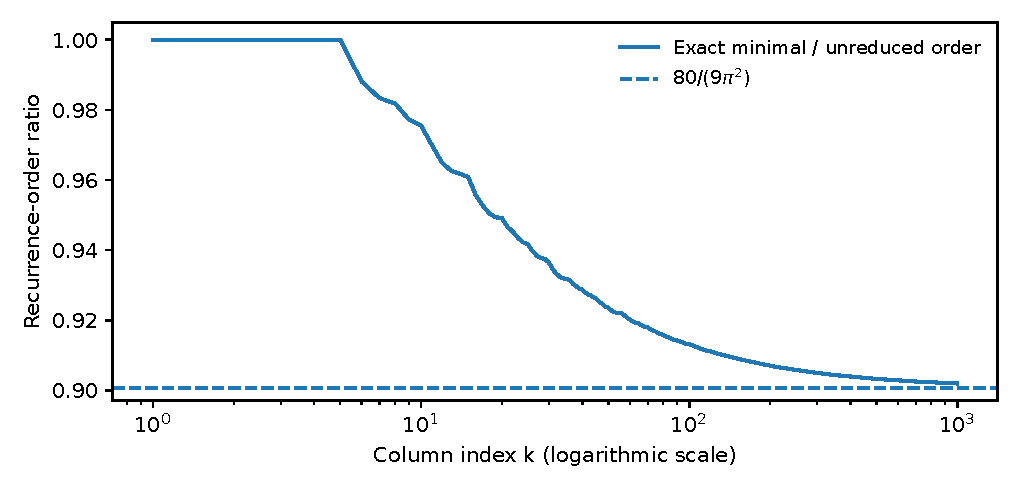
\includegraphics[width=.91\linewidth]{data/order_ratio.pdf}
\caption{The recurrence-order ratio computed from the exact totient formula,
not from numerical root finding.  The dashed line is the proved limit.}
\label{zz:fig:ratio}
\end{figure}

\section{Consequences and corrections for the OEIS entries}
\label{zz:sec:oeis}
This section concerns presentation and indexing in the entries retrieved on
1 October 2026; it does not claim the underlying fixed-column formulas as new.

\subsection{The product denominator is not generally reduced}
The first collision is between $D_1$ and $D_7$:
\[
 D_1=1-x,\qquad
 D_7=(x-1)(x^2-x-1)(x^4+x^3-4x^2-4x+1).
\]
Consequently,
\[
 R_6=\mathcal P_6/(1-x),\qquad r_6=83<84,
\]
and
$R_7=\mathcal P_7/(1-x)^2$, $r_7=118<120$.
The latter cancellation was already noticed in \cite[Remark~5.7]{xz}.
\Cref{zz:thm:factorization} gives the complete all-column replacement for a
case-by-case cancellation check.

\subsection{A numerator-degree index shift}
A005586 has value $a(u)=u(u+4)(u+5)/6$ at index~$u$ \cite{oeis5586}.
The unreduced numerator degree in \eqref{zz:eq:old-num} is therefore
\[
 \deg G_k=\mathrm{A005586}(k-1)\qquad(k\ge1),
\]
not $\mathrm{A005586}(k)$ as the literal zero-based wording of Conjecture~4(ii)
in A205497 suggests.  For example, $G_1=1$ has degree~$0$, not~$5$.
The explicit polynomial degree formula itself is already present in
\cite{xz}; this is an indexing correction to the entry, not a new degree theorem.

\subsection{The sign of the last coefficient in column three}
The numerator of $C_3$ is
\begin{align}\label{zz:eq:N3}
 N_3(x)={}&1+x-6x^2-15x^3+21x^4+35x^5-13x^6-51x^7\notag\\
 &+3x^8+21x^9+5x^{10}+x^{11}-5x^{12}-x^{13}+x^{14}.
\end{align}
The final sign is \emph{positive}.  The formula in A205497's Conjecture~5.4
has a negative sign at $x^{14}$ \cite{oeis205497}; the positive sign is already
printed in \cite[Example~5.11]{xz}.
The discrepancy first changes the coefficient of $x^{14}$ in the generating
function, since the common denominator has constant term~$1$:
\[
 [x^{14}]C_3(x)=M_{14,3}=z(19,3)=546629054.
\]
The negative-sign version gives $546629052$.  The former also agrees with
the independently listed A205493 term \cite{oeis205493}.
The supplied code verifies the exact difference $2x^{14}$ between the two
numerators, rather than silently replacing the source data.

\subsection{The known limit as a corollary of a stronger expansion}
The Chebyshev expression in the old column-ratio conjecture equals
\begin{equation}\label{zz:eq:ratio-old}
 \rho_{k+1}=\frac1{2\sin(\pi/(4k+6))}
 =U_k\left(\cos\frac{\pi}{2k+3}\right).
\end{equation}
Indeed, $U_k(\cos\beta)=\sin((k+1)\beta)/\sin\beta$, and
$(k+1)\beta=\pi/2-\beta/2$ for $\beta=\pi/(2k+3)$.
The positive coefficient $\alpha_{k+1}$ proves the corresponding ratio limit.
The next section supplies error estimates and secondary terms rather than
reclaiming this established limit.

\section{Uniform spectral estimates}
\label{zz:sec:uniform}
\subsection{Bounds independent of matrix size}
The key simplification is that the leading eigenvalue dominates all other
ones by a factor bounded away from~$1$, uniformly in the alphabet size.

\begin{lemma}[Uniform order-polynomial estimate]
\label{zz:lem:uniform-omega}
For every $m,n\ge1$,
\begin{equation}\label{zz:eq:omega-uniform}
 \left|\frac{\Om_n(m)}{\alpha_m\rho_m^n}-1\right|
 \le4\,2^{-n}.
\end{equation}
Also
\begin{equation}\label{zz:eq:uniform-constants}
 \frac3\pi\le\alpha_m\le\frac43,\qquad
 0<\Om_n(m)\le\frac\pi2\rho_m^n.
\end{equation}
\end{lemma}
\begin{proof}
For $m\ge2$, the ratio of the second-largest eigenvalue in absolute value to
$\rho_m$ is
\[
 \frac{\sin t_m}{\sin3t_m}
 =\frac1{3-4\sin^2t_m}<\frac12,
\]
since $t_m\le\pi/10<\pi/6$.
The orthogonal spectral decomposition and $\|\one\|^2=m$ give
\[
 |\Om_n(m)-\alpha_m\rho_m^n|
 \le m(\rho_m/2)^{n-1}.
\]
Because $m/\rho_m=2m\sin t_m\le2mt_m<\pi/2$, division by
$\alpha_m\rho_m^n$ gives the desired bound once the amplitude bounds are
established.  Now
\[
 \alpha_m=\frac4\pi\frac{t_m\cos^2t_m}{\sin t_m},\qquad
 0<t_m\le\pi/6.
\]
The inequalities $\sin t\le t$, $\cos^2t\ge3/4$, and
$\sin t\ge3t/\pi$ on this interval give
$3/\pi\le\alpha_m\le4/3$.
Thus $m/(\alpha_m\rho_m)\le\pi^2/6$ and the spectral relative error is
at most $(\pi^2/3)2^{-n}<4\,2^{-n}$.
The norm bound $|\one^TH_m^{n-1}\one|\le m\rho_m^{n-1}$ gives the final
upper bound.  When $m=1$, the approximation is exact and all inequalities hold.
\end{proof}

\subsection{Concavity of the logarithmic growth rate}
Extend the formulas for $\rho_m$ and $\alpha_m$ to real $u\ge1$.
Write $y=u+1/2$, $t=\pi/(4y)$, and
\[
 f(u)=\log\rho_u,\qquad g(u)=\log\alpha_u,\qquad
 \delta_u=f'(u)=\frac{t\cot t}{y}.
\]

\begin{lemma}[Derivative bounds]
\label{zz:lem:derivatives}
For $u\ge1$,
\begin{equation}\label{zz:eq:deriv-bounds}
 \begin{gathered}
 f'(u)>0,\qquad
 -\frac2{(u+1/2)^2}\le f''(u)\le-\frac1{2(u+1/2)^2},\\
 |g''(u)|\le\frac7{(u+1/2)^2}.
 \end{gathered}
\end{equation}
In particular, for integers $1\le m\le M$,
\begin{equation}\label{zz:eq:eigen-ratio}
 \rho_m/\rho_M\le e^{-(M-m)\delta_M}.
\end{equation}
As $u\to\infty$,
\begin{equation}\label{zz:eq:delta-asympt}
 \delta_u=\frac1{u+1/2}+O(u^{-3}).
\end{equation}
\end{lemma}
\begin{proof}
Direct differentiation gives
\[
 y^2f''(u)=t^2\csc^2t-2t\cot t.
\]
On $0<t\le\pi/6$, one has
$t/\sin t\le\pi/3$ and $t\cot t\ge\cos t\ge\sqrt3/2$.
Therefore
$y^2f''\le\pi^2/9-\sqrt3<-1/2$.
The lower bound $y^2f''\ge-2$ follows from $t\cot t\le1$ and
$t^2\csc^2t\ge0$.
For the amplitude, write
\[
 g(u)=\log(4/\pi)+h(t),\qquad
 h(t)=\log(t/\sin t)+2\log\cos t.
\]
A second differentiation gives
\[
 y^2g''(u)=1-2t\cot t-4t\tan t+t^2\csc^2t-2t^2\sec^2t.
\]
Its absolute value is at most
\[
 1+2+\frac{2\pi}{3\sqrt3}+\frac{\pi^2}{9}
    +\frac{2\pi^2}{27}<7.
\]
Since $f'$ is decreasing, integrating it from $m$ to $M$ yields
\eqref{zz:eq:eigen-ratio}.  Finally $t\cot t=1+O(t^2)$ proves
\eqref{zz:eq:delta-asympt}.
\end{proof}

\subsection{An explicit relative-error bound}
\begin{theorem}[Uniform coefficient approximation]
\label{zz:thm:uniform-bound}
For $n\ge1$, $k\ge0$, $M=k+1$, and $q=e^{-n\delta_M}$,
\begin{equation}\label{zz:eq:error-exact}
 \left|\frac{z(n,k)}{\alpha_M\rho_M^n}-1\right|
 \le4\,2^{-n}+2\bigl((1+q)^{n+1}-1\bigr).
\end{equation}
If $(n+1)q\le1$, the right side is at most
\begin{equation}\label{zz:eq:error-simple}
 E(n,M):=4\,2^{-n}+4(n+1)e^{-n\delta_M}.
\end{equation}
For every fixed $0<c<1$, this error tends to zero uniformly for
$M\le c n/\log n$.
\end{theorem}
\begin{proof}
Separate the $j=0$ term in \eqref{zz:eq:extraction}.  Its relative error is bounded
by \cref{zz:lem:uniform-omega}.  For $j\ge1$, the upper bound in
\eqref{zz:eq:uniform-constants}, the lower bound on $\alpha_M$, and
\eqref{zz:eq:eigen-ratio} give
\[
 \frac{\binom{n+1}{j}\Om_n(M-j)}{\alpha_M\rho_M^n}
 \le\frac{\pi^2}{6}\binom{n+1}{j}q^j
 <2\binom{n+1}{j}q^j.
\]
Sum absolute values, extending to the full binomial sum.
If $(n+1)q\le1$, use
$(1+q)^{n+1}-1\le e^{(n+1)q}-1\le2(n+1)q$.

For uniformity, $\delta_u$ decreases with $u$.
At the largest permitted size $L=c n/\log n$,
\[
 n\delta_L=\frac{\log n}{c}+o(1).
\]
Consequently $(n+1)e^{-n\delta_M}\le n^{1-1/c+o(1)}\to0$
uniformly over $M\le L$.  This also guarantees the hypothesis for the simpler
bound once $n$ is sufficiently large.
\end{proof}

This proves part~(i) of \cref{zz:thm:main-analysis}.  It also shows why the fixed
column limit by itself is not enough for shape questions: the growing
binomial coefficients in \eqref{zz:eq:extraction} must be controlled uniformly.

\subsection{Two spectral terms for fixed columns}
\begin{proposition}
\label{zz:prop:two-term}
For each fixed $k\ge2$,
\begin{equation}\label{zz:eq:two-term}
 z(n,k)=\alpha_{k+1}\rho_{k+1}^{n}
 -(n+1)\alpha_k\rho_k^n
 +O_k(n^2\rho_{k-1}^n).
\end{equation}
For $k=1$ the exact formula is
$z(n,1)=F_{n+2}-(n+1)$, where $F_0=0,F_1=1$ are the Fibonacci numbers.
\end{proposition}
\begin{proof}
The Perron terms at $m=k+1$ and $m=k$ in \eqref{zz:eq:exp-poly} give the two
terms displayed.  The Perron term at $m=k-1$ is of order
$n^2\rho_{k-1}^n$.  Every Perron term at a smaller size has a strictly smaller
exponential base, so its fixed polynomial factor can be absorbed in that
bound.  Among all non-Perron eigenvalues with $m\le k+1$, the largest
absolute value is $1/(2\sin(3\pi/(4k+6)))$, and
\[
 \frac1{2\sin(3\pi/(4k+6))}
 <\frac1{2\sin(\pi/(4k-2))}=\rho_{k-1}
 \qquad(k\ge2).
\]
Indeed the two angles lie in $(0,\pi/2)$ and the first is larger.
All remaining spectral terms are therefore absorbed as well.
For $k=1$, use $\Om_n(2)=F_{n+2}$ and $\Om_n(1)=1$ in
\eqref{zz:eq:extraction}.
\end{proof}

\section{The crossover at \texorpdfstring{$k\asymp n/\log n$}{k of order n/log n}}
\label{zz:sec:crossover}
The uniform bound identifies a transition scale.  At that scale it is no
longer correct simply to discard all terms with $j\ge1$ in
\eqref{zz:eq:extraction}.  Their combined effect has a closed limiting form.

\begin{theorem}[Crossover law]
\label{zz:thm:crossover}
Let $k=k(n)$ be nonnegative integers such that
\begin{equation}\label{zz:eq:crossover-hyp}
 s_n:=\frac{n}{k+3/2}-\log n\longrightarrow s\in\R.
\end{equation}
Then
\begin{equation}\label{zz:eq:crossover-limit}
 \frac{z(n,k)}{\alpha_{k+1}\rho_{k+1}^n}\longrightarrow e^{-e^{-s}}.
\end{equation}
Equivalently,
\begin{equation}\label{zz:eq:crossover-elementary}
 z(n,k)\sim\frac4\pi
 \left(\frac{2k+3}{\pi}\right)^n e^{-e^{-s}}.
\end{equation}
\end{theorem}
\begin{proof}
Put $M=k+1$.  The hypothesis implies $M\sim n/\log n$, so
$n/M^2\to0$, and \eqref{zz:eq:delta-asympt} gives
\[
 n\delta_M-\log n=s_n+o(1)\to s.
\]
For a fixed $j\ge0$, Taylor expansion of $f=\log\rho$ on
$[M-j,M]$ gives
\[
 n\bigl(f(M-j)-f(M)\bigr)
 =-nj\delta_M+O_j(n/M^2).
\]
Also $\alpha_{M-j}/\alpha_M\to1$, and
\cref{zz:lem:uniform-omega} is uniform in the changing size $M-j$.
It follows that the absolute value of the $j$th normalized summand in
\eqref{zz:eq:extraction} tends to $e^{-js}/j!$.

To justify summing these limits, define summands to be zero for $j\ge M$.
For all $j\ge0$, the same estimate used in \cref{zz:thm:uniform-bound} gives
\[
 \frac{\binom{n+1}{j}\Om_n(M-j)}{\alpha_M\rho_M^n}
 \le2\frac{((n+1)e^{-n\delta_M})^j}{j!}
 \quad(0\le j<M).
\]
The quantity $(n+1)e^{-n\delta_M}$ stays bounded.  Thus a fixed summable
majorant $2K^j/j!$ applies for all sufficiently large $n$.
Dominated convergence for the series yields
\[
 \lim\frac{z(n,k)}{\alpha_M\rho_M^n}
 =\sum_{j=0}^\infty\frac{(-e^{-s})^j}{j!}=e^{-e^{-s}}.
\]
Finally, $\alpha_M\to4/\pi$ and
\[
 \rho_M=\frac{2M+1}{\pi}\bigl(1+O(M^{-2})\bigr).
\]
Since $n/M^2\to0$, taking the $n$th power leaves a relative factor tending
to~$1$.  This proves \eqref{zz:eq:crossover-elementary}.
\end{proof}

The function $e^{-e^{-s}}$ is the familiar Gumbel distribution function.
Here it appears as a \emph{deterministic relative coefficient correction};
no claim of a random-variable limit law is needed.
At $s=0$ the correction is $e^{-1}$, rather than~$1$.
Thus the theorem describes precisely a regime where an unqualified leading
Perron approximation would have a persistent relative error.

\begin{corollary}
\label{zz:cor:simple-asympt}
If $k/\sqrt n\to\infty$ and $k\log n/n\to0$, then
\[
 z(n,k)\sim\frac4\pi\left(\frac{2k+3}{\pi}\right)^n.
\]
\end{corollary}
\begin{proof}
Use \cref{zz:thm:uniform-bound}, $\alpha_{k+1}\to4/\pi$, and
$n/(k+1)^2\to0$ in the expansion of $\rho_{k+1}$.
\end{proof}

\section{A growing part of the log-concavity conjecture}
\label{zz:sec:logconcavity}
It is essential to distinguish uniformity in $k$ from a separate eventual
statement for every fixed $k$.  The theorem below supplies the former.

\begin{lemma}[Curvature of the leading approximation]
\label{zz:lem:leading-curvature}
For every integer $m\ge2$ and $n\ge160$,
\begin{equation}\label{zz:eq:leading-curvature}
 \log\frac{(\alpha_m\rho_m^n)^2}
 {\alpha_{m-1}\rho_{m-1}^n\,\alpha_{m+1}\rho_{m+1}^n}
 \ge\frac{n}{4(m+3/2)^2}.
\end{equation}
\end{lemma}
\begin{proof}
For any twice continuously differentiable function $h$,
\[
 2h(m)-h(m-1)-h(m+1)
 =-\int_{-1}^1(1-|v|)h''(m+v)\,dv.
\]
Apply \cref{zz:lem:derivatives} to $h=nf+g$.  The result is bounded below by
\[
 \frac{n}{2(m+3/2)^2}-\frac7{(m-1/2)^2}.
\]
For $m\ge2$, $(m+3/2)/(m-1/2)\le7/3$, so the last expression is at least
\[
 \frac{n/2-343/9}{(m+3/2)^2}\ge\frac{n}{4(m+3/2)^2}
 \quad(n\ge160).
\]
\end{proof}

\begin{theorem}[Growing-edge strict log-concavity]
\label{zz:thm:edge-lc}
Fix $0<c<1/2$.  There exists $n_0(c)$ such that every $n\ge n_0(c)$ and
integer $k\ge1$ with $k+2\le cn/\log n$ satisfy
\[
 z(n,k)^2>z(n,k-1)z(n,k+1).
\]
For the same $n$, this also holds at $n-2-k$.
\end{theorem}
\begin{proof}
Let $L=cn/\log n$ and consider all three alphabet sizes
$k,k+1,k+2\le L$ simultaneously.  By \cref{zz:thm:uniform-bound}, their
relative errors are at most
\[
 E_L=4\,2^{-n}+4(n+1)e^{-n\delta_L}.
\]
For sufficiently large $n$, $E_L<1/2$.  Since
$|\log(1+u)|\le2|u|$ for $|u|\le1/2$, the difference between the actual
log-concavity logarithm and the leading one in
\eqref{zz:eq:leading-curvature} has absolute value at most $8E_L$.
Consequently the actual logarithm is at least
\begin{equation}\label{zz:eq:lc-lower}
 \frac{n}{4(k+5/2)^2}-8E_L.
\end{equation}
The ratio of the second term to a constant multiple of the first is bounded
by a constant times
\[
 \frac{(L+1/2)^2}{n}E_L
 =O\bigl(n\,2^{-n}\bigr)
   +O\left(L^2e^{-n\delta_L}\right)
 =n^{2-1/c+o(1)}\,O((\log n)^{-2})+o(1).
\]
This tends to zero because $c<1/2$.
Thus \eqref{zz:eq:lc-lower} is positive uniformly over all allowed $k$.
The reflected statement follows from \eqref{zz:eq:symmetry}.
\end{proof}

\begin{remark}[What is and is not resolved]
\label{zz:rem:not-full}
The theorem proves infinitely many inequalities in a region whose width
increases like $n/\log n$.  It is strictly stronger than eventual
log-concavity at each fixed distance from an edge.
However, the width is still $o(n)$; the theorem does not reach a fixed
positive fraction of a row or its center.  It therefore does not settle
Petersen--Zhuang Conjecture~6.1(b) in full.  It does not prove real-rootedness,
simple roots, or an interlacing/Sturm property either.
\end{remark}

\begin{corollary}[Every fixed edge index]
For each fixed integer $k\ge1$,
\[
 \frac{z(n,k)^2}{z(n,k-1)z(n,k+1)}
 \sim\frac{\alpha_{k+1}^2}{\alpha_k\alpha_{k+2}}
 \left(\frac{\rho_{k+1}^2}{\rho_k\rho_{k+2}}\right)^n,
\]
and this quotient tends to infinity.
\end{corollary}
\begin{proof}
Apply the fixed-index cases of \cref{zz:thm:uniform-bound}.
Strict concavity of $\log\rho_u$ implies
$\rho_{k+1}^2>\rho_k\rho_{k+2}$.
\end{proof}

\section{Reproducible exact checks and numerical diagnostics}
\label{zz:sec:verification}
The accompanying scripts use no network access.  Their roles are deliberately
separated: integer and rational identities test algebraic implementation,
while floating-point evaluations illustrate analytic results.

\subsection{Exact checks}
The default run of \texttt{verify.py} (shipped as \texttt{code/verify.py})
completed the following checks:
\begin{enumerate}[label=(\arabic*)]
\item Direct symbolic determinants agree with \eqref{zz:eq:D-recurrence} for
$m=1,\ldots,9$.  Exact polynomial gcds agree with \cref{zz:thm:gcd} for all
$820$ unordered pairs $1\le m,n\le40$.
\item Direct enumeration of weak alternating words agrees with the matrix
walk count for $m=1,\ldots,4$ and $n=0,\ldots,6$.  Direct enumeration of
alternating permutations and their big returns agrees with the extracted
triangle for $n=0,\ldots,9$.
\item Exact numerator and reduced-denominator certificates are produced for
columns $k=0,\ldots,12$.  Each pair is checked for coprimality, the predicted
degrees, and at least $2r_k+26$ independently computed coefficients.
\item All rows through $n=100$ were checked for symmetry, positivity, and
log-concavity.  These finite row checks are evidence only, not a proof of the
full conjecture.  The specified OEIS numerator discrepancy is also tested.
\end{enumerate}
No check failed in the final run.  The initial comparison against the printed
column-three numerator detected the sign discrepancy explained in
\cref{zz:sec:oeis}; the final test records that discrepancy explicitly.

The certificates are in \texttt{data/rational\_certificates.json}, with
coefficients in ascending powers of $x$.
The file \texttt{data/minimal\_orders.txt} gives $r_k$ for $0\le k\le1000$.
It is candidate sequence data, not a claim that a new OEIS identifier has
been assigned.  The full machine-readable result is
\texttt{data/verification\_report.json}.

\subsection{How the rational certificates are constructed}
For $F_m=E_m/D_m$, one may avoid large symbolic expression simplifications.
For $j\ge1$,
\begin{equation}\label{zz:eq:derivative-certificate}
 \sum_{n\ge0}\binom{n+1}{j}\Om_n(m)x^n
 =\frac{x^{j-1}}{j!}\frac{d^j}{dx^j}\bigl(xF_m(x)\bigr).
\end{equation}
Start with numerator $S=xE_m$ and denominator $D_m^p$, $p=1$.
One differentiation updates
\[
 S\longmapsto S'D_m-pSD_m',\qquad p\longmapsto p+1.
\]
After $j$ steps, multiply by $x^{j-1}/j!$.
For column $k$, multiply each resulting numerator by the exact polynomial
quotient $R_k/D_m^{k+2-m}$, sum with alternating signs, and divide by
$x^{k+2}$.  This produces $N_k$ using only exact polynomial arithmetic.
The $j=0$ and $k=0$ cases are handled separately as above.

For coefficient verification, a suffix-sum multiplication by $H_m$ takes
$O(m)$ integer additions.  Thus all $\Om_n(m)$ with $n\le N$ and $m\le M$
can be generated in $O(NM^2)$ additions.  This is an arithmetic-operation
count; large integer bit lengths must still be included in a bit-complexity
analysis.  A recurrence built from $R_k$ is useful for a long fixed column,
but the approximate $9.94\%$ degree reduction alone does not establish the
best wall-clock algorithm.

\subsection{Uniform-approximation diagnostics}
\Cref{zz:tab:asymptotic} uses exact integer $z(n,k)$ and high-precision evaluation
of the formulas.  The error-bound column evaluates the rigorous expression
\eqref{zz:eq:error-exact}, but its decimal evaluation is not interval-certified.
\begin{table}[ht]
\centering\small
\caption{Relative Perron errors and log-concavity logarithms.  The last column
is $\log(z(n,k)^2/(z(n,k-1)z(n,k+1)))$.}
\begin{tabular}{rrrrr}
\toprule
$n$ & $k$ & Actual relative error & Bound expression & Logarithm\\
\midrule
50 & 2 & 3.622e-06 & 8.108e-05 & 4.044101 \\
100 & 5 & 6.153e-06 & 4.534e-05 & 2.361166 \\
200 & 10 & 2.598e-06 & 1.156e-05 & 1.511073 \\
500 & 20 & 2.303e-08 & 8.044e-08 & 1.081403 \\
1000 & 40 & 2.562e-08 & 6.883e-08 & 0.580597 \\
2000 & 80 & 3.786e-08 & 8.812e-08 & 0.301098 \\
\bottomrule
\end{tabular}
\label{zz:tab:asymptotic}
\end{table}

\subsection{Crossover diagnostics}
\Cref{zz:tab:crossover} illustrates \cref{zz:thm:crossover}.  Let
$W=z(n,k)/(\alpha_{k+1}\rho_{k+1}^n)$.  For these larger sizes we compute its
finite alternating Perron sum, rather than construct the enormous exact
integer.  The omitted tail and the non-Perron contribution have explicit
analytic bounds; floating-point roundoff is a separate issue, and the table
is only a numerical diagnostic.

Specifically, put $K=(n+1)e^{-n\delta_M}$ and retain $0\le j<100$.
The absolute analytic remainder is at most
\[
 2e^K\frac{K^{100}}{100!}+8\,2^{-n}e^K.
\]
The first term bounds the factorial tail; the second follows from the uniform
spectral bound.  These are not bounds on the error of replacing $W$ by the
\emph{limiting} crossover prediction.
\begin{table}[ht]
\centering\small
\caption{Approach to the crossover correction.  Here $s_n=n/(k+3/2)-\log n$;
$W$ is evaluated by the truncated Perron sum.}
\begin{tabular}{rrrrr}
\toprule
$n$ & $k$ & $s_n$ & $W$ & $e^{-e^{-s_n}}$\\
\midrule
1000 & 168 & -1.00805 & 0.05858841 & 0.06455401 \\
1000 & 143 & 0.01266 & 0.37213775 & 0.37253665 \\
1000 & 125 & 0.99738 & 0.69634269 & 0.69153368 \\
10000 & 1216 & -0.99679 & 0.06547651 & 0.06656577 \\
10000 & 1084 & 0.00200 & 0.36856637 & 0.36861673 \\
10000 & 978 & 0.99895 & 0.69274428 & 0.69193318 \\
100000 & 9511 & -1.00044 & 0.06573410 & 0.06590880 \\
100000 & 8684 & 0.00052 & 0.36806410 & 0.36806944 \\
100000 & 7990 & 1.00037 & 0.69241787 & 0.69229481 \\
\bottomrule
\end{tabular}
\label{zz:tab:crossover}
\end{table}

\section{A formalization route for ProveIt}
\label{zz:sec:formalization}
A practical formalization should keep three boundaries separate.
\paragraph{Finite combinatorics and algebra.}
Define weak alternating words, the matrix $H_m$, and the suffix-sum evaluator.
Prove their counting equivalence and then the descent/order-polynomial
identity.  A finite polynomial checker can verify each concrete pair
$(N_k,R_k)$ using rational arithmetic.  This finite layer does not require
trigonometric analysis.
\paragraph{Uniform algebraic structure.}
Formalize the sine eigenvectors or an equivalent Chebyshev description,
including the nonzero projection of $\one$ onto every eigenspace.
The noncancellation argument is then a general lemma about finite sums of
exponential-polynomial sequences with distinct multiplier degrees.
The gcd formula and first-occurrence factor theorem provide the structural
content that finite examples cannot certify.
\paragraph{Analysis.}
The derivative inequalities, explicit error estimate, dominated convergence
for the crossover, and finite-difference curvature bound can be developed
independently of a full theory of roots of zig-zag Eulerian polynomials.
Their statements should retain quantifiers over growing index ranges;
replacing a uniform theorem by a pointwise limit would lose the essential
content of \cref{zz:thm:edge-lc}.

The included files are not untested Lean code presented as a formal proof.
A future formalization should report exactly which of these boundaries has
been crossed, and which imported results or analytic facts remain assumptions.

\section{Further research questions}
\label{zz:sec:questions}
The results suggest several concrete projects.  They are deliberately stated
as questions or proposed programs, not as established consequences.

\subsection{Full-row log-concavity and its central regime}
Can the growing-edge theorem be joined to a local limit or saddle-point
analysis valid when $k/n$ stays in a compact subinterval of $(0,1)$?
A pointwise central approximation is insufficient: the error must be smaller
than the second finite difference of the logarithm of the main term.
An overlap theorem would be especially valuable because it could establish
eventual full-row log-concavity, after which a finite certificate might handle
the remaining rows.  Neither step has been supplied here.

\subsection{Beyond the constant \texorpdfstring{$1/2$}{1/2} in the edge theorem}
The restriction $c<1/2$ comes from bounding the three logarithmic errors
separately.  It is a limitation of this estimate, not an identified phase
transition in log-concavity.  Can one control the \emph{second difference of
the error} directly?  The crossover formula suggests that the individual
errors may vary smoothly enough for much better cancellation in that second
difference.  An explicit theorem for $c\ge1/2$ is a well-defined next target.

\subsection{A quantitative crossover expansion}
Prove a rate and additional terms in \cref{zz:thm:crossover}, uniformly for $s_n$
in a fixed compact interval.  The fixed-$j$ expansion involves
$n j^2/(k+3/2)^2$, which is of order $(\log n)^2/n$ at crossover.
One can expect the next terms to arise from exponential sums of $j$, $j^2$,
and higher powers against $(-e^{-s})^j/j!$.
A useful result would give an explicit uniform remainder, not just fitted
coefficients.  The finite-index rounding of $k$ must be retained through $s_n$.

\subsection{A direct combinatorial meaning of the crossover correction}
The exponential series in the proof resembles a sieve over rare defects.
Is there a combinatorial construction whose limiting exclusion probability
is $e^{-e^{-s}}$ and whose exact count is $z(n,k)$ after normalization?
Such a construction could explain the correction without relying solely on
signed coefficient extraction, and might lead to estimates deeper inside the
triangle.

\subsection{Sharper recurrence-order asymptotics}
The current remainder $O(k^2\log k)$ is enough to identify the leading
constant but does not resolve a secondary term.  The exact totient sum reduces
the problem to weighted odd-totient summatory estimates.
Can one describe the secondary behavior, including any arithmetic
fluctuations, with a useful explicit error?
A correct answer must not infer a polynomial second term from a short table.

\subsection{Minimal realizations and fast exact generation}
The degree $r_k$ determines the minimum linear state dimension over a field,
but a dense recurrence need not be the fastest realization over the integers.
Can the factor decomposition in \eqref{zz:eq:Rfactor} be exploited by modular
polynomial arithmetic, block recurrences, or rational reconstruction?
The target is a proved bit-complexity bound and a reproducible comparison
against suffix-sum dynamic programming, with output size accounted for.

\subsection{Other periodic fence orientations}
Replace the alternating orientation by a fixed periodic pattern of up and
down comparisons.  The order-polynomial transfer matrix becomes a product of
upper and lower summation matrices.
Which patterns retain an explicit spectrum, and which permit a first-occurrence
classification strong enough to determine every fixed-descent minimal
recurrence?  The noncancellation principle from \cref{zz:sec:minimal} survives
whenever the spectral weights and the polynomial multipliers can be controlled;
the difficult part is identifying and comparing the spectra.

\subsection{Real-rootedness and refined interlacing}
The full real-rootedness conjecture remains separate from the present
argument.  A direct stability-preserving recurrence, an interlacing refinement,
or a sign-regular matrix model would be stronger than gamma-positivity alone.
The refined recurrences of \cite{pz} provide a concrete starting point, but
an assertion that they preserve real roots requires a proof of every needed
interlacing hypothesis.  The current spectral formulas concern the index $n$
in fixed columns and do not automatically control zeros in the descent
variable~$t$.

\section{Conclusion}
The fixed-column theory of A205497 has an exact algebraic refinement: its
minimum recurrence is controlled by the \emph{earliest appearance} of each
reciprocal eigenvalue, not by multiplying all available denominators.
That observation yields a complete collision classification and an explicit
cubic order constant.

The same spectral representation has a second use.  Uniform control of
alphabet size makes it possible to pass from fixed-column asymptotics to a
crossover law and to strict log-concavity in a growing edge region.
The remaining central and real-rootedness questions are clearly delimited.
The package supplies ordinary proofs, exact reproducible computations, and
specific next problems; it does not convert limited checks or a literature
search into a claim of a fully formalized or globally priority-certified
breakthrough.

\appendix
\section{A finite, explicit log-concavity certificate from the bounds}
\label{zz:app:finite-criterion}
The existence statement in \cref{zz:thm:edge-lc} can be used without guessing
$n_0(c)$.  For given integers $n\ge160$ and $k\ge1$, put $L=k+2$ and
$q_L=e^{-n\delta_L}$.  If
\begin{equation}\label{zz:eq:finite-criterion}
 (n+1)q_L\le1,\quad E(n,L)<\frac12,\quad
 8E(n,L)<\frac{n}{4(k+5/2)^2},
\end{equation}
then $z(n,k)^2>z(n,k-1)z(n,k+1)$.
Indeed, the errors at all three sizes are bounded by $E(n,L)$ because
$\delta_u$ decreases, and \eqref{zz:eq:lc-lower} is positive.
These inequalities involve elementary real functions only; an interval
implementation could make a formally checkable numerical certificate for
specific ranges.  The decimal diagnostics supplied here do not implement
that interval certification.

\section{Package contents and reproduction}
\label{zz:app:package}
The main source is \texttt{zigzag\_spectral\_research.tex}; its bibliography is
embedded below, so no external bibliography database is required.
\begin{verbatim}
python verify.py --out-dir data
python illustrate.py
latexmk -pdf -interaction=nonstopmode -halt-on-error \
    zigzag_spectral_research.tex
\end{verbatim}
\texttt{build.sh} executes these steps.  Python dependencies are SymPy,
mpmath, and Matplotlib; the final recorded run used Python~3.13.5,
SymPy~1.14.0, and mpmath~1.3.0.
The exact checks can be rerun separately from \texttt{illustrate.py}.
The generated plot, small typeset tables, machine-readable certificates,
triangle values, and numerical diagnostics are in \texttt{data/}.
No font files or external copyrighted articles are included.

\emph{[Write note, batch 73O2, 1 October 2026.]} The paragraph above
describes the delivered package. In ProveIt the source is
\texttt{article.tex}, the scripts and both build wrappers are in
\texttt{code/}, and the recorded outputs and \texttt{requirements.txt} are
in \texttt{data/}. The delivered commands, and \texttt{build.sh} and
\texttt{build.ps1}, rewrite the recorded files in \texttt{data/}, and after
the move \texttt{code/verify.py} by default writes to \texttt{code/data/};
the report's \texttt{README.md} gives commands that run on a copy. The
figure \texttt{data/order\_ratio.pdf} was regenerated from the unmodified
\texttt{illustrate.py} with TrueType instead of Type~3 fonts; its content is
unchanged (see the README).

\section{Provenance}
\label{zz:sec:provenance}
This report is one manuscript, number~36 of batch 73O2 of ProveIt's
incoming-reports intake: the archive \texttt{zigzag\_oeis\_research.zip}
(main file \texttt{zigzag\_spectral\_research.tex}, 22-page PDF), dated
1 October 2026, which arrived in commit \texttt{f8c3a392a} and was placed by
commit \texttt{6e193dd4f}. It cites no repository revision: its only
repository source is the ProveIt README, inspected on 1 October 2026. The
text is as delivered except for the label prefix \texttt{zz:}, the citation
of A050446 (listed but uncited in the delivered bibliography) in
Section~\ref{zz:sec:definitions}, the shipped path of the verification
script in Section~\ref{zz:sec:verification}, this appendix, the
repository bibliography entry, and the dated write notes in
Section~\ref{zz:sec:intro} and Appendix~\ref{zz:app:package}.

\begin{thebibliography}{9}
\bibitem{oeis205497}
The OEIS Foundation, \emph{A205497: Triangle read by rows: Zig-zag Eulerian
number triangle $T(n,k)$}.  Entry and internal-format comments retrieved
1 October 2026. \url{https://oeis.org/A205497}.

\bibitem{oeis50446}
The OEIS Foundation, \emph{A050446}.  Order-polynomial / weak alternating-word
array, with indexing conventions reconciled in the cited papers.
\url{https://oeis.org/A050446}.

\bibitem{oeis5586}
The OEIS Foundation, \emph{A005586: $a(n)=n(n+4)(n+5)/6$}.
Retrieved 1 October 2026. \url{https://oeis.org/A005586}.

\bibitem{oeis205493}
The OEIS Foundation, \emph{A205493: Third row or column of table A205497}.
Retrieved 1 October 2026. \url{https://oeis.org/A205493}.

\bibitem{xz}
G. Xin and Y. Zhong, \emph{Proving some conjectures on Kekul\'e numbers for
certain benzenoids by using Chebyshev polynomials}, Advances in Applied
Mathematics \textbf{145} (2023), Article 102479.
The theorem and example numbering used here refers to the accessible
arXiv version, arXiv:2201.02376v1 (2022).
\url{https://arxiv.org/abs/2201.02376}.

\bibitem{pz}
T. K. Petersen and Y. Zhuang, \emph{Zig-zag Eulerian polynomials},
European Journal of Combinatorics \textbf{124} (2025), Article 104073.
Accessible version: arXiv:2403.07181v4, 9 September 2024.
\url{https://arxiv.org/abs/2403.07181}.

\bibitem{proveit}
V. Reshetnikov, \emph{ProveIt}, repository README, inspected 1 October 2026.
\url{https://github.com/VladimirReshetnikov/ProveIt}.

\bibitem{cti}
ProveIt, \emph{Combinatorial Transseries and Their Inverses},
\nolinkurl{Analysis/Transseries/docs/series-and-transseries/Combinatorial_Transseries_Inverses/}.
Cited in the write
(batch 73O2), not by the manuscript.
\end{thebibliography}
\end{document}
